%!TEX root = slides.tex
%!TEX program = xelatex
% (für das LaTeXtools Sublime plugin)

\documentclass{beamer}

%Blablabla front matter....

\title{Quantum Key Distribution}
\subtitle{Foundational Aspects of Quantum Mechanics}
\date{01-02-2017}
\author[Hirscher, Snijders]{Simon Hirscher \& Max Snijders}

%\setbeameroption{show notes}
%\setbeamertemplate{note page}[plain]

\usepackage[LastSlideNotCounted,ProgressBar,NoPageCounter]{beamer-template-mk-i/beamerthememxmki}
\hypersetup{pdfpagemode=FullScreen}

% Use this for the handout!

% \usepackage{pgfpages}
% \pgfpagesuselayout{4 on 1}[a4paper]

% Quotes are awesome! (Sometimes)

\newcommand*{\openquote}{\tikz[remember picture,overlay,xshift=-15pt,yshift=-10pt]
	\node (OQ) {\fontsize{60}{60}\selectfont``};\kern0pt}
\newcommand*{\closequote}{\tikz[remember picture,overlay,xshift=15pt,yshift=10pt]
	\node (CQ) {\fontsize{60}{60}\selectfont''};}
% select a colour for the shading
\definecolor{shadecolor}{named}{white}
% wrap everything in its own environment
\newenvironment{shadequote}%
{\begin{quote}\openquote}
		{\hfill\closequote\end{quote}}


% And now for the real deal...
\begin{document}
	% commented out so it doesn't appear in the table of contents
	%\section{Introduction} % Simon
	\begin{frame}
		\begin{center}
		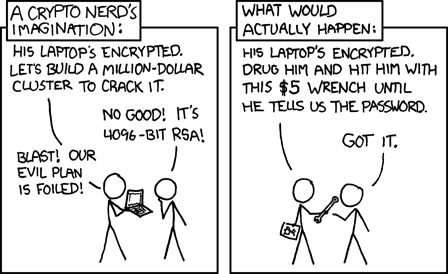
\includegraphics[width=0.8\textwidth]{images/xkcd-security.png}
		\end{center}
	\end{frame}

	\begin{frame}
		\titlepage
	\end{frame}

	% Structure of the talk
	\begin{frame}{Contents} % Simon
		\tableofcontents
	\end{frame}

	\section{Introduction to Encryption}
	\begin{frame}{The setting}
		Alice and Bob
	\end{frame}

	\begin{frame}{What is Encryption?} % Simon
		\begin{equation}
			\operatorname{ENC}: \underset{\cong\;\mathbb{N}}{\{\text{plaintexts}\}}
						\overset{\text{bijective}}{\longrightarrow}
						\underset{\cong\;\mathbb{N}}{\{\text{ciphertexts}\}}\nonumber
		\end{equation}
		\begin{itemize}
			\item The function should be easily reversible for the
			recipient but impossible to reverse for a 3rd party

 			\item \textbf{Symmetric encryption:} $\operatorname{ENC}$
 			and $\operatorname{ENC}^{-1}$ are generated from one secret
 			number, referred to as \textbf{the shared secret} or
 			\textbf{secret key}.

 			\item \textbf{Asymmetric encryption:} $\operatorname{ENC}$
 			is generated from a \textbf{public key}, known to everyone
 			and specific to the recipient, $\operatorname{ENC}^{-1}$
 			generated from a \textbf{private key}, known only to the
 			recipient.

		\end{itemize}
	\end{frame}

	\begin{frame}{Shifting Caesar Cipher} % Max
		\begin{columns}
			\begin{column}{0.7\textwidth}
				\begin{figure}
					\begin{tikzpicture}[scale=1, every node/.style={scale=1}]
					    \node[anchor=center,inner sep=0] at (-0.08,-0.00) {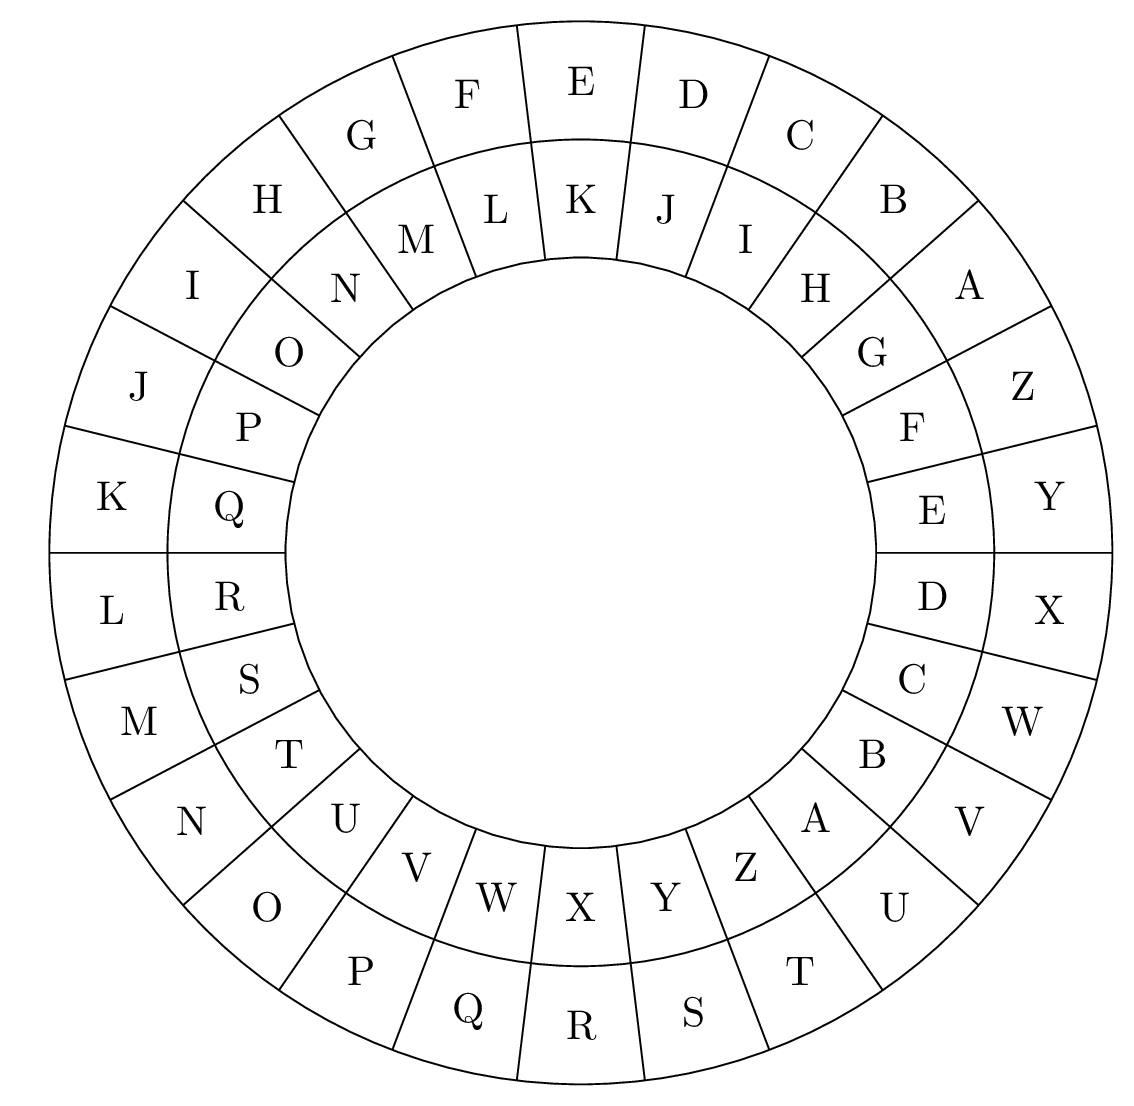
\includegraphics[width=0.85\textwidth]{images/shifting-caesar-cipher}};

					    \draw[fill = Bordeaux, thick] (0,0) circle(0.1);

					    \onslide<3->{\draw[Bordeaux, thick,->, opacity=0.5] (0:0) -- (48.5:2.37);}
						\onslide<2->{\draw[Bordeaux, ultra thick,->,opacity=1.0] (0:0) -- (48.5:1.69);}

						\onslide<5->{\draw[Bordeaux, thick,->, opacity=0.5] (0:0) -- (6.9:2.37);}
						\onslide<4->{\draw[Bordeaux, ultra thick,->,opacity=1.0] (0:0) -- (6.9:1.69);}

						\onslide<7->{\draw[Bordeaux, thick,->, opacity=0.5] (0:0) -- (103.8:2.37);}
						\onslide<6->{\draw[Bordeaux, ultra thick,->,opacity=1.0] (0:0) -- (103.8:1.69);}

						\onslide<9->{\draw[Bordeaux, thick,->, opacity=0.5] (0:0) -- (145.4:2.37);}
						\onslide<8->{\draw[Bordeaux, ultra thick,->,opacity=1.0] (0:0) -- (145.4:1.69);}
					\end{tikzpicture}
				\end{figure}
			\end{column}
			\begin{column}{0.3\textwidth}
				\begin{itemize}
					\onslide<10->\item 26 options
					\onslide<11->\item Vulnerable to brute-force attack.
				\end{itemize}
			\end{column}
		\end{columns}
	\end{frame}

	\begin{frame}{Permutation Cipher} % Max
		\begin{columns}
			\begin{column}{0.5\textwidth}
				\begin{figure}
					\begin{table}
						\begin{tabular}{ c | c }
							Plaintext & Ciphertext \\
							\hline \\
							\onslide<2->{A & G \\}
							\onslide<3->{B & X \\}
							\onslide<4->{C & C \\}
							\onslide<5->{D & J \\}
							\onslide<6->{\vdots & \vdots}
						\end{tabular}
					\end{table}
				\end{figure}
			\end{column}
			\begin{column}{0.5\textwidth}
				\begin{itemize}
					\onslide<7->\item $26 \cdot 25 \cdot 24 \cdot \hdots \cdot 1 = 26! \approx 10^{26}$ options
					\onslide<8->\item Vulnerable to frequency analysis.
				\end{itemize}
			\end{column}
		\end{columns}
	\end{frame}

	\begin{frame}{XOR} % Simon

	\end{frame}

	\begin{frame}{One-Time Pad} % Simon

	\end{frame}

	% Key distribution section
	\section{Key Distribution}

	\begin{frame}{Diffie-Hellman Key Exchange (DHE)} % Max
		\begin{columns}
			\begin{column}{\textwidth}
				\begin{figure}
					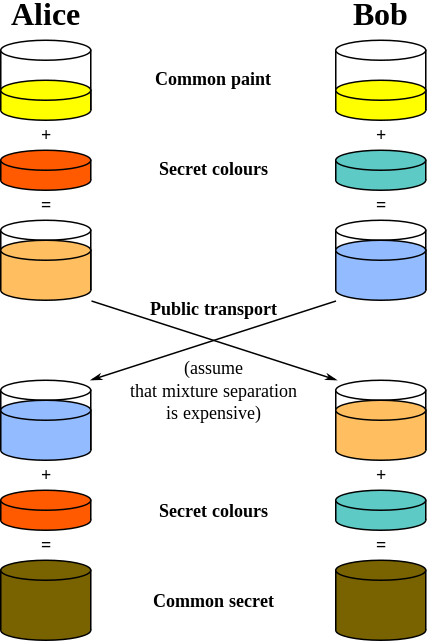
\includegraphics[width=0.4\textwidth]{images/diffie-hellman}
				\end{figure}
			\end{column}
		\end{columns}
	\end{frame}

	\begin{frame}{Public/Private Key} % Simon

	\end{frame}

	% Methods of Quantum Key Exchange
	\section{Quantum Key Distribution}

	\begin{frame}{BB-84} % Max

	\end{frame}

	\begin{frame}{E-91} % Simon

	\end{frame}

	% Authentication Requirement
	\section{Authentication}

	\begin{frame}{Public/Private Key Authentication} % Simon

	\end{frame}

	% Hacks
	\section{Vulnerabilities}

	\begin{frame}{Vulnerabilities} % Max
		\begin{itemize}
			\item Sender basis detection
		\end{itemize}
	\end{frame}

	% Closing
	\section{Closing}

	\begin{frame}
		\begin{center}
		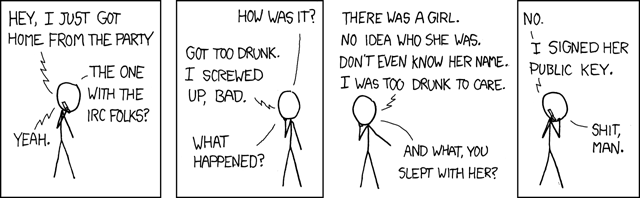
\includegraphics[width=\textwidth]{images/xkcd-responsible_behavior}
		\end{center}
	\end{frame}


	% A black slide to end the talk
	\setbeamercolor{background canvas}{bg=black}
	\begin{frame}[plain]\end{frame}

\end{document}